\documentclass[aspectratio=169]{beamer}
\mode<presentation>
\usepackage{panqueques}
\usepackage[brazil]{babel}
\usepackage{svg}
\usepackage{booktabs}
\usepackage[font=footnotesize,labelfont=bf]{caption}
% Acrônimos e Cores da Disciplina de Cálculo Numérico
\definecolor{pblue}{rgb}{0.13,0.13,1}
\definecolor{javagreen}{rgb}{0,0.5,0}
\definecolor{javapurple}{rgb}{0.5,0,0.35}
\definecolor{javadocblue}{rgb}{0,0.33,0.93}
\definecolor{backcolour}{rgb}{0.95,0.95,0.92}
\definecolor{codegreen}{rgb}{0,0.6,0}
\definecolor{codegray}{rgb}{0.5,0.5,0.5}
\definecolor{codepurple}{rgb}{0.58,0,0.82}

\usepackage{inconsolata}
\usepackage{listings}
\usepackage{hyperref}
\usepackage[normalem]{ulem}

% ============================================================
% CONFIGURAÇÃO DE CORES E ESTILOS
% ============================================================
\definecolor{primary}{RGB}{26, 115, 232}
\definecolor{secondary}{RGB}{234, 67, 53}
\definecolor{accent}{RGB}{52, 168, 83}
\definecolor{background}{RGB}{248, 249, 250}
\definecolor{codebg}{RGB}{245, 245, 245}
\definecolor{commentcolor}{RGB}{0, 128, 0}
\definecolor{backcolour}{rgb}{0.96,0.96,0.94}
\definecolor{codegreen}{rgb}{0,0.55,0}
\definecolor{codegray}{rgb}{0.45,0.45,0.45}
\definecolor{codepurple}{rgb}{0.58,0,0.82}

\lstdefinestyle{pythonstyle}{
    backgroundcolor=\color{backcolour},
    commentstyle=\color{codegreen}\itshape,
    keywordstyle=\color{primary}\bfseries,
    numberstyle=\tiny\color{codegray},
    stringstyle=\color{codepurple},
    basicstyle=\ttfamily\scriptsize,
    breakatwhitespace=false,
    breaklines=true,
    captionpos=b,
    keepspaces=true,
    numbers=left,
    numbersep=4pt,
    showspaces=false,
    showstringspaces=false,
    showtabs=false,
    tabsize=2,
    language=Python,
    extendedchars=true,
    morekeywords={as, True, False, None, np, linspace, exp, sum, abs, sqrt, ceil}
}
\lstset{style=pythonstyle}

\usepackage{algorithm}
\usepackage[noend]{algpseudocode}
\usepackage{verbatim}
\usepackage{multirow}
\usepackage{tikz}
\usetikzlibrary{shapes.geometric,shapes.multipart,arrows.meta,positioning,fit,backgrounds,decorations.pathreplacing,calc,shadows,trees}

% Estilos TikZ para Diagramas Numéricos e Fluxogramas
\tikzset{
    boxnode/.style={rectangle, draw=primary!80!black, fill=primary!10, thick, rounded corners, align=center, font=\scriptsize\bfseries},
    actnode/.style={rectangle, draw=accent!80!black, fill=accent!15, thick, rounded corners, align=center, font=\scriptsize},
    errnode/.style={rectangle, draw=secondary!80!black, fill=secondary!15, thick, rounded corners, align=center, font=\scriptsize},
    flowedge/.style={thick, draw=gray!80!black, -{Stealth[length=2.5mm]}}
}

\usepackage[backend=bibtex, style=numeric, sorting=none]{biblatex}
\addbibresource{3-reference/ref.bib}

% ============================================================
% COMANDOS PERSONALIZADOS
% ============================================================
\newcommand{\highlight}[1]{\textcolor{primary}{\textbf{#1}}}
\newcommand{\emphred}[1]{\textcolor{secondary}{\textbf{#1}}}
\newcommand{\emphgreen}[1]{\textcolor{accent}{\textbf{#1}}}
\newcommand{\code}[1]{\texttt{#1}}

% ============================================================
% INFORMAÇÕES DO DOCUMENTO
% ============================================================
\title{Integração Numérica: Método dos Trapézios\\Das Fórmulas de Newton-Cotes à Implementação em Python}
\author{Prof. João Cardoso}
\date{\today}

\begin{document}

% Página de Título
\begin{frame}[noframenumbering,plain, allowframebreaks]
    \begin{tikzpicture}[remember picture, overlay]
        \fill[red!70!black] (current page.south west) rectangle ([xshift=4cm]current page.north west);
        %\node at ([xshift=2cm,yshift=-4.5cm]current page.north west) %{\includegraphics[width=3cm]{1-title-page/logo-cin.png}};
    \end{tikzpicture}
    \begingroup  
        \flushright
        {\fontfamily{qag}\selectfont\Large\bfseries\color{red!70!black}\MyTitle}\vspace{1em}\\
        \MyAuthor\vspace{0.5em}\\
        \MyDate\par
    \endgroup
\end{frame}

%edit as needed

% ------------------------------------------------------------
% ROTEIRO DA AULA
% ------------------------------------------------------------
\begin{frame}[plain]
    \begingroup
        \fontfamily{qag}\selectfont
        \Huge\color{red!70!black}\textbf{Sumário da Aula}\\[0.6em]
    \endgroup
    \begingroup
        \tableofcontents
    \endgroup
\end{frame}

% ============================================================
% SEÇÃO 1: MOTIVAÇÃO E O GUARDA-CHUVA DA INTEGRAÇÃO NUMÉRICA
% ============================================================
\section{Motivação e Recapitulação de Newton-Cotes}

\begin{frame}{Motivação: Por que Estudar Integração Numérica?}
\footnotesize
Calcular $I = \int_a^b f(x)\,dx$ pelo Teorema Fundamental do Cálculo ($F(b) - F(a)$) falha ou torna-se impraticável em dois cenários centrais da Ciência e Engenharia \cite{santos2010, mesquita2026, burden2016}:

\begin{columns}[T]
\begin{column}{0.5\textwidth}
\begin{bee}[\small Cenários de Aplicação Inevitável]
\begin{itemize}\scriptsize
    \item \textbf{1. Função Desconhecida (Dados Tabulados)}: Possuímos apenas um conjunto discreto de medições $(x_i, f(x_i))$ coletadas por sensores, ensaios laboratoriais ou séries temporais.
    \item \textbf{2. Primitiva Impossível ou Inviável}: A função $f(x)$ é conhecida analiticamente, mas não possui antiderivada elementar em forma fechada (ex.: $\int_a^b e^{-x^2}\,dx$, $\int_a^b \frac{\sin x}{x}\,dx$, $\int_a^b \sqrt{1 + \cos^2 x}\,dx$).
\end{itemize}
\end{bee}
\end{column}

\begin{column}{0.5\textwidth}
\begin{bee}[\small Aplicações Reais na Computação e Engenharia]
\begin{itemize}\scriptsize
    \item \textbf{Física e Engenharia}: Cálculo de trabalho mecânico ($\int F(x)\,dx$), deslocamento a partir de velocímetros e fluxo térmico.
    \item \textbf{Probabilidade e Estatística}: Avaliação de probabilidades acumuladas em distribuições contínuas (Normal, Weibull).
    \item \textbf{Ciência de Dados e IA}: Cálculo da métrica \highlight{AUC-ROC} (área sob a curva ROC) via regra dos trapézios no \code{scikit-learn} e análise de sinais \cite{chapra2016, scipy_trapezoid}.
\end{itemize}
\end{bee}
\end{column}
\end{columns}
\end{frame}

\begin{frame}{Recapitulação: Fórmulas de Newton-Cotes sob o Guarda-Chuva Numérico}
\footnotesize
Na aula anterior, vimos que a estratégia unificadora das \highlight{Fórmulas Fechadas de Newton-Cotes} consiste em particionar $[a, b]$ em $n$ subintervalos iguais de passo $h = \frac{b - a}{n}$, com nós $x_k = x_0 + kh$ ($x_0 = a, x_n = b$), e integrar o \highlight{polinômio interpolador de Lagrange} $P_n(x)$ \cite{santos2010, ruggiero1996, mesquita2026}:
\[
\int_{x_0}^{x_n} f(x)\,dx = \int_{x_0}^{x_n} \left[\sum_{k=0}^{n} L_k^n(x) f(x_k) + R_n(x)\right]\,dx = \sum_{k=0}^{n} C_k^n f(x_k) + T, \quad C_k^n = \frac{(-1)^{n-k}h}{k!(n-k)!}\int_0^n \frac{\pi_n(z)}{z-k}\,dz
\]
\vspace{-0.25cm}
\begin{center}
\begin{tikzpicture}[scale=0.85, transform shape]
    \node[boxnode, fill=red!12, draw=red!70!black, minimum width=5.6cm] (guarda) at (0, 1.55) {INTEGRAÇÃO NUMÉRICA (Quadratura)\\Substituir $f(x)$ por um polinômio interpolador $P_n(x)$};
    \node[boxnode, minimum width=4.8cm] (nc) at (0, 0.35) {Fórmulas de Newton-Cotes ($x_k = x_0 + kh$, $z = \frac{x - x_0}{h}$)};
    \node[actnode, minimum width=3.5cm, draw=primary, fill=primary!15] (trap) at (-4.4, -1.05) {\textbf{Grau $n = 1$ (Retas)}\\Método dos Trapézios\\{\tiny (Aula de Hoje)}};
    \node[boxnode, minimum width=3.5cm] (simp13) at (0, -1.05) {\textbf{Grau $n = 2$ (Parábolas)}\\Regra $1/3$ de Simpson\\{\tiny (Próxima Aula)}};
    \node[boxnode, minimum width=3.5cm] (simp38) at (4.4, -1.05) {\textbf{Grau $n = 3$ (Cúbicas)}\\Regra $3/8$ de Simpson\\{\tiny (Próxima Aula)}};

    \draw[flowedge] (guarda) -- (nc);
    \draw[flowedge] (nc.south) -- ++(0,-0.25) -| (trap.north);
    \draw[flowedge] (nc.south) -- (simp13.north);
    \draw[flowedge] (nc.south) -- ++(0,-0.25) -| (simp38.north);
\end{tikzpicture}
\end{center}
\end{frame}

% ============================================================
% SEÇÃO 2: FORMALISMO MATEMÁTICO DO MÉTODO DOS TRAPÉZIOS
% ============================================================
\section{Formalismo Matemático do Método dos Trapézios}

\begin{frame}{Conexão Direta: Newton-Cotes ($n=1$) $\rightarrow$ Trapézio Simples}
\footnotesize
Tomando $n = 1$ na fórmula geral de Newton-Cotes sobre um único subintervalo $[x_0, x_1]$ de largura $h = x_1 - x_0$, temos $\pi_1(z) = z(z - 1)$ e os dois pesos de Cotes são deduzidos analiticamente \cite{santos2010, mesquita2026}:

\begin{columns}[T]
\begin{column}{0.52\textwidth}
\begin{bee}[\small Dedução dos Coeficientes $C_0^1$ e $C_1^1$]
\begin{itemize}\scriptsize
    \item Para $k = 0$:
    \[
    C_0^1 = \frac{(-1)^1 h}{0!\,1!} \int_0^1 (z - 1)\,dz = -h \left[\frac{z^2}{2} - z\right]_0^1 = \frac{h}{2}
    \]
    \item Para $k = 1$:
    \[
    C_1^1 = \frac{(-1)^0 h}{1!\,0!} \int_0^1 z\,dz = h \left[\frac{z^2}{2}\right]_0^1 = \frac{h}{2}
    \]
\end{itemize}
\end{bee}
\end{column}

\begin{column}{0.48\textwidth}
\begin{bee}[\small Regra do Trapézio Simples e Motivação Composta]
\begin{itemize}\scriptsize
    \item Substituindo os pesos, obtemos a área do trapézio de altura $h$ e bases $f(x_0)$ e $f(x_1)$:
    \[
    \int_{x_0}^{x_1} f(x)\,dx = \frac{h}{2}\big[f(x_0) + f(x_1)\big] + T_1
    \]
    \item \emphred{Por que subdividir em vez de elevar $n$ global?} Polinômios de grau alto sofrem com o \textbf{Fenômeno de Runge} (oscilações espúrias nas bordas) e geram coeficientes $C_k^n < 0$ para $n \ge 8$ \cite{ruggiero1996, burden2016}.
\end{itemize}
\end{bee}
\end{column}
\end{columns}
\end{frame}

\begin{frame}{Interpretação Geométrica: Trapézio Simples vs. Composto}
\footnotesize
Em vez de aproximar $f(x)$ por uma única reta secante em $[a, b]$, o \highlight{Método dos Trapézios Composto} particiona o domínio em $n$ subintervalos $[x_i, x_{i+1}]$ e soma as áreas de cada trapézio elementar:

\begin{center}
    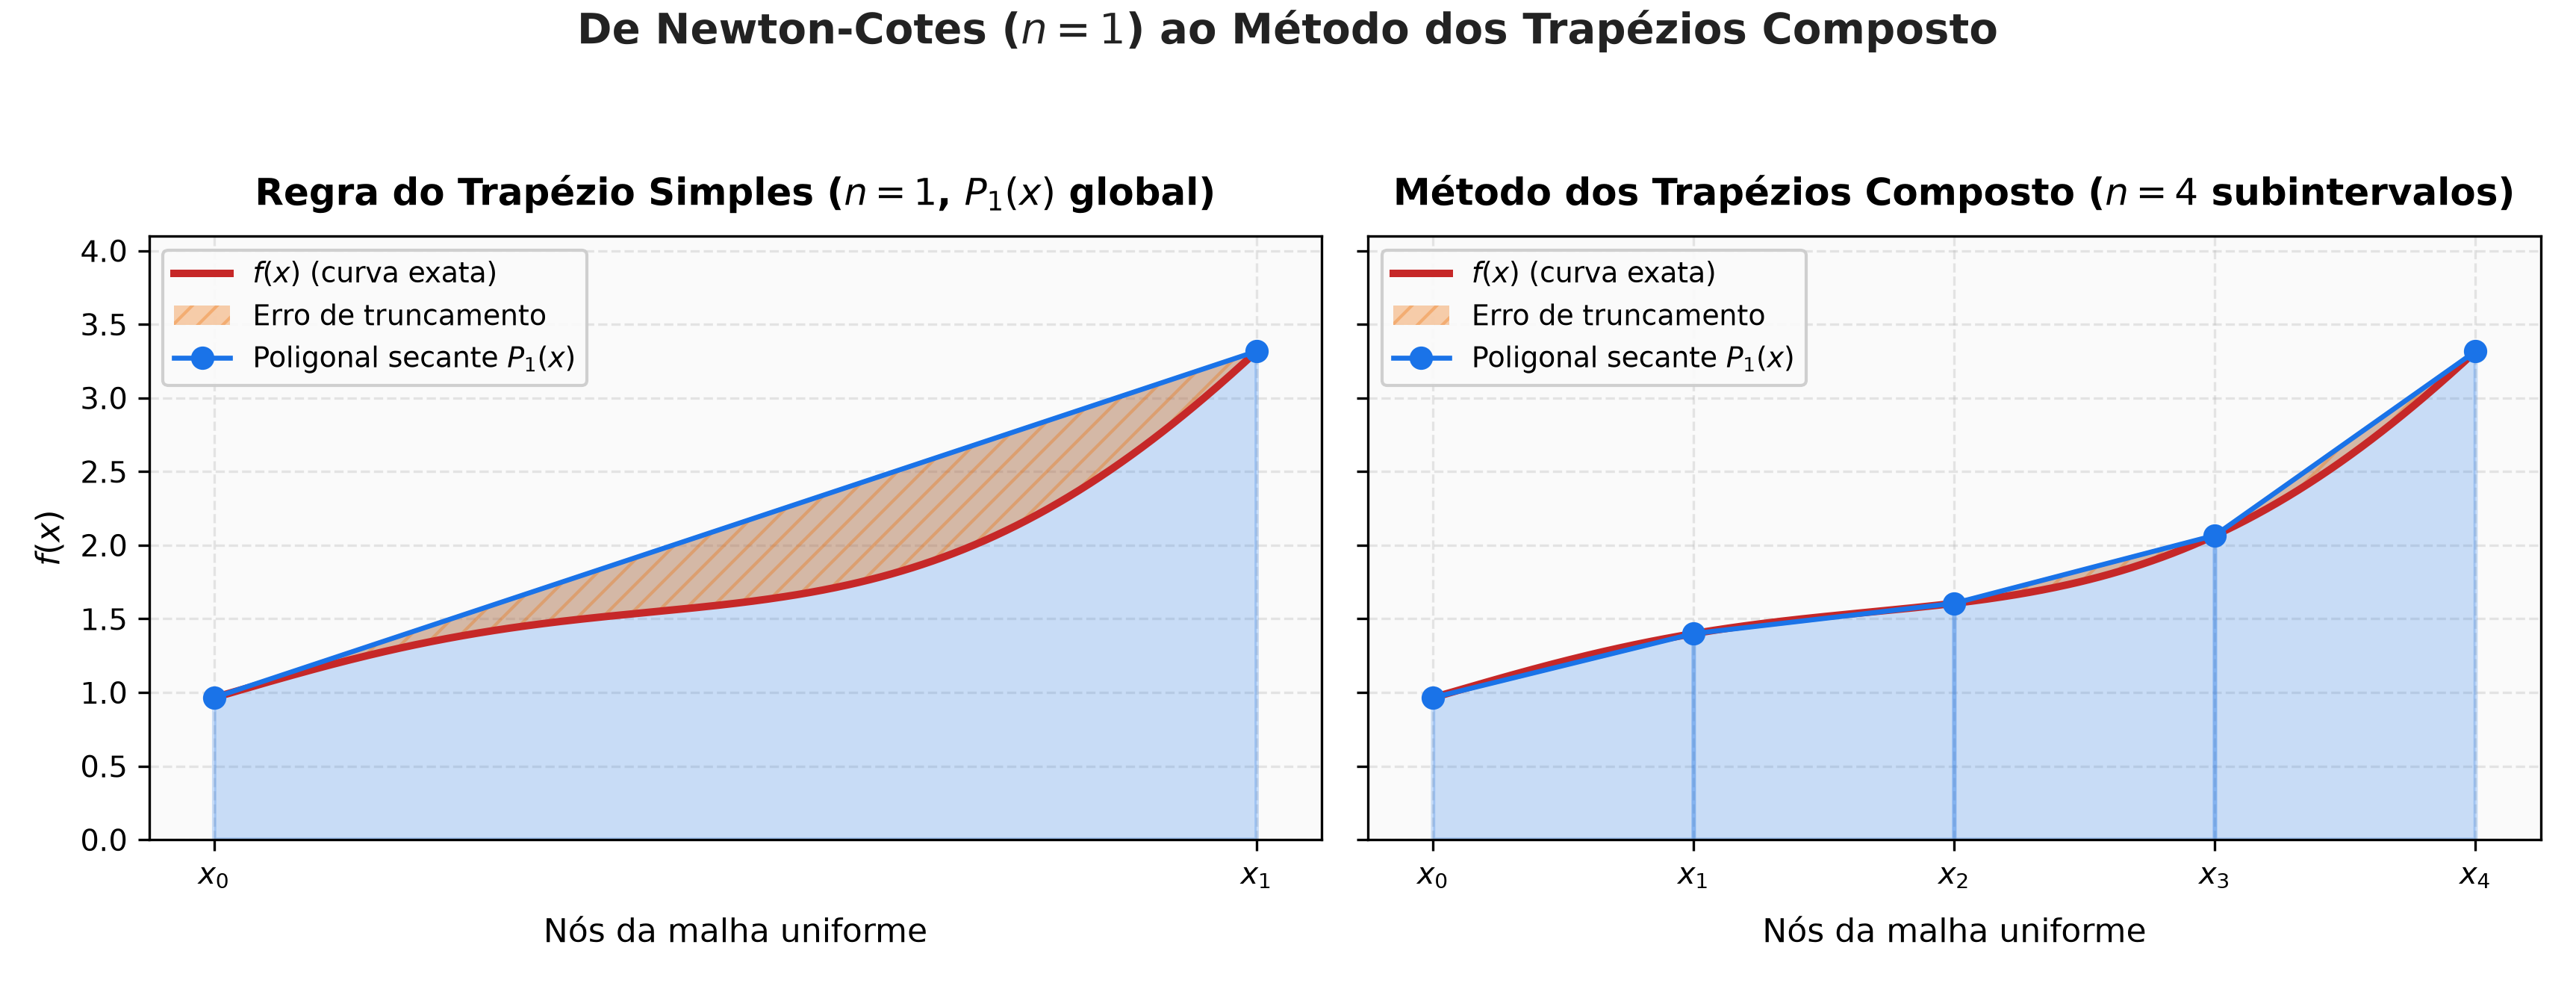
\includegraphics[width=0.92\linewidth]{images/fig_newton_cotes_trapezio.png}
\end{center}
\vspace{-0.25cm}
\begin{center}
    \tiny Figura gerada em Python: redução drástica da região de erro (hachurada) ao passar de $n=1$ para $n=4$ \cite{cardoso2026_github}.
\end{center}
\end{frame}

\begin{frame}{Dedução do Método dos Trapézios Composto (Generalizado)}
\footnotesize
Dividindo $[a, b] = [x_0, x_n]$ em $n$ subintervalos iguais de passo $h = \frac{x_n - x_0}{n}$ e aplicando a propriedade aditiva da integral definida \cite{santos2010, claudio1994, mesquita2026}:
\[
\int_{x_0}^{x_n} f(x)\,dx = \sum_{i=0}^{n-1} \int_{x_i}^{x_{i+1}} f(x)\,dx = \sum_{i=0}^{n-1} \left( \frac{h}{2}\big[f(x_i) + f(x_{i+1})\big] + T_{i+1} \right)
\]
Cada nó interno $x_1, x_2, \dots, x_{n-1}$ participa de \highlight{dois trapézios adjacentes} ($\frac{h}{2} + \frac{h}{2} = h$), enquanto os extremos $x_0$ e $x_n$ participam de apenas um ($\frac{h}{2}$):

\begin{columns}[T]
\begin{column}{0.56\textwidth}
\begin{bee}[\small Fórmula Canônica e Agrupamento Operacional]
\[
\int_{x_0}^{x_n} f(x)\,dx = h \left[ \frac{f(x_0) + f(x_n)}{2} + \sum_{i=1}^{n-1} f(x_i) \right] + T_t \approx h\left(\frac{E}{2} + I + P\right)
\]
\begin{itemize}\tiny
    \item $E = f(x_0) + f(x_n)$: soma das imagens nos \textbf{extremos}.
    \item $I = \sum_{\text{ímpar}} f(x_i)$ e $P = \sum_{\text{par}} f(x_i)$: internos (sem extremos).
\end{itemize}
\end{bee}
\end{column}

\begin{column}{0.44\textwidth}
\begin{bee}[\small Vantagens e Limitações Práticas]
\begin{itemize}\scriptsize
    \item \emphgreen{Vantagem}: Aplica-se a \textbf{qualquer} $n \ge 1$ (par ou ímpar) e apresenta alta estabilidade numérica (todos os pesos positivos).
    \item \emphred{Desvantagem}: Convergência mais lenta que Simpson quando $f$ é muito suave e possui curvatura acentuada \cite{ruggiero1996}.
\end{itemize}
\end{bee}
\end{column}
\end{columns}
\end{frame}

\begin{frame}{Análise do Erro de Truncamento e Ordem de Convergência}
\footnotesize
Integrando o resto da interpolação linear $R_1(x) = \frac{f''(\eta(x))}{2}(x - x_i)(x - x_{i+1})$ em cada subintervalo $[x_i, x_{i+1}]$ (via Teorema do Valor Médio Ponderado para Integrais), obtemos o erro local $T_{i+1} = -\frac{h^3}{12}f''(\eta_i)$ \cite{burden2016, ruggiero1996}:

\begin{columns}[T]
\begin{column}{0.54\textwidth}
\begin{bee}[\small Erro Global e Cota Máxima Teórica]
Somando os $n$ erros locais e usando $nh = b - a$:
\[
T_t = -\frac{n h^3}{12} f''(\xi) = -\frac{(b - a) h^2}{12} f''(\xi), \quad \xi \in (a, b)
\]
Logo, definindo $M_2 = \max_{x \in [a, b]} |f''(x)|$:
\[
\textcolor{primary}{|T_t| \le \frac{n h^3}{12} M_2 = \frac{(b - a)^3}{12 n^2} M_2}
\]
\end{bee}
\end{column}

\begin{column}{0.46\textwidth}
\begin{bee}[\small Propriedades Analíticas Fundamentais]
\begin{itemize}\scriptsize
    \item \textbf{Ordem de Convergência $O(h^2)$}: Reduzir o passo $h$ pela metade (dobrar $n$) divide o erro por $4$.
    \item \textbf{Grau de Precisão 1}: Se $f(x)$ for reta ($f'' \equiv 0$), $T_t = 0$ (resultado exato).
    \item \textbf{Concavidade}: $f'' > 0 \Rightarrow T_t < 0$ (superestima); $f'' < 0 \Rightarrow T_t > 0$ (subestima).
    \item \textbf{Dimensionamento}: Para erro $\le \varepsilon$, escolha:
    \[
    n \ge \left\lceil \sqrt{\frac{(b - a)^3 M_2}{12 \varepsilon}} \right\rceil
    \]
\end{itemize}
\end{bee}
\end{column}
\end{columns}
\end{frame}

% ============================================================
% SEÇÃO 3: EXERCÍCIO RESOLVIDO PASSO A PASSO
% ============================================================
\section{Exercício Resolvido Passo a Passo}

\begin{frame}{Exercício Resolvido (Parte 1): Cálculo de $\int_{0,0}^{0,6} e^x\,dx$ com 7 Pontos}
\footnotesize
\textbf{Enunciado} \cite{santos2010, mesquita2026}: Calcule aproximadamente $\int_{0,0}^{0,6} e^x\,dx$ pelo Método dos Trapézios usando \textbf{7 pontos} no intervalo $[0{,}0;\; 0{,}6]$ e compare com o valor exato $I_{\text{exato}} = e^{0{,}6} - e^{0{,}0} \approx 0{,}82211880$.

\begin{columns}[T]
\begin{column}{0.48\textwidth}
\begin{center}
\scriptsize
\begin{tabular}{cccc}
\toprule
$i$ & $x_i$ & $f(x_i) = e^{x_i}$ & Grupo \\
\midrule
0 & $0{,}0$ & $1{,}00000000$ & Extremo ($E$) \\
1 & $0{,}1$ & $1{,}10517092$ & Ímpar ($I$) \\
2 & $0{,}2$ & $1{,}22140276$ & Par ($P$) \\
3 & $0{,}3$ & $1{,}34985881$ & Ímpar ($I$) \\
4 & $0{,}4$ & $1{,}49182470$ & Par ($P$) \\
5 & $0{,}5$ & $1{,}64872127$ & Ímpar ($I$) \\
6 & $0{,}6$ & $1{,}82211880$ & Extremo ($E$) \\
\bottomrule
\end{tabular}
\end{center}
\end{column}

\begin{column}{0.52\textwidth}
\begin{bee}[\small Passo a Passo da Resolução]
\begin{itemize}\scriptsize
    \item \textbf{Passo}: 7 pontos $\Rightarrow n = 6$ subintervalos $\Rightarrow h = \frac{0{,}6 - 0{,}0}{6} = 0{,}1$.
    \item \textbf{Somas parciais}:
    \begin{align*}
        E &= f(x_0) + f(x_6) = 2{,}82211880 \;\Rightarrow\; \frac{E}{2} = 1{,}41105940 \\
        I &= f(x_1) + f(x_3) + f(x_5) = 4{,}10375100 \\
        P &= f(x_2) + f(x_4) = 2{,}71322746
    \end{align*}
    \item \textbf{Aproximação Numérica}:
    \[
    I_T = 0{,}1 \times \left(1{,}41105940 + 4{,}10375100 + 2{,}71322746\right) = \textcolor{primary}{\mathbf{0{,}82280379}}
    \]
    \item Observe que $I_T > I_{\text{exato}}$ pois $f''(x) = e^x > 0$ (concavidade para cima).
\end{itemize}
\end{bee}
\end{column}
\end{columns}
\end{frame}

\begin{frame}{Exercício Resolvido (Parte 2): Cota Máxima do Erro vs. Erro Real}
\footnotesize
Utilizando o mesmo enunciado anterior ($\int_{0,0}^{0,6} e^x\,dx$ com $n = 6$ subintervalos e $h = 0{,}1$), determine a \highlight{cota máxima do erro de truncamento} $|T_t|$ e confronte com o erro real cometido \cite{santos2010, mesquita2026}.

\begin{columns}[T]
\begin{column}{0.52\textwidth}
\begin{bee}[\small Estimativa Teórica a Priori ($M_2$)]
\begin{enumerate}\scriptsize
    \item Calculamos a segunda derivada da função integranda:
    \[
    f(x) = e^x \;\Rightarrow\; f'(x) = e^x \;\Rightarrow\; f''(x) = e^x
    \]
    \item Como $e^x$ é estritamente crescente em $[0{,}0;\; 0{,}6]$:
    \[
    M_2 = \max_{x \in [0{,}0;\; 0{,}6]} |e^x| = e^{0{,}6} \approx 1{,}82211880
    \]
    \item Aplicando a fórmula da cota do erro:
    \[
    |T_t| \le \frac{n h^3}{12} M_2 = \frac{6 \times (0{,}1)^3 \times e^{0{,}6}}{12} = \textcolor{primary}{\mathbf{9{,}1105940 \times 10^{-4}}}
    \]
\end{enumerate}
\end{bee}
\end{column}

\begin{column}{0.48\textwidth}
\begin{bee}[\small Confronto com o Erro Real Observado]
\begin{itemize}\scriptsize
    \item Valor analítico exato:
    \[
    I_{\text{exato}} = e^{0{,}6} - 1 = 0{,}82211880
    \]
    \item Erro absoluto real:
    \[
    |E_{\text{real}}| = |0{,}82211880 - 0{,}82280379| = 6{,}849848 \times 10^{-4}
    \]
    \item \emphgreen{Validação teórica}:
    \[
    6{,}8498 \times 10^{-4} \le 9{,}1106 \times 10^{-4} \quad (\text{garantido!})
    \]
    \item A cota garante com folga $3$ casas decimais exatas antes mesmo de conhecer a solução analítica.
\end{itemize}
\end{bee}
\end{column}
\end{columns}
\end{frame}

% ============================================================
% SEÇÃO 4: IMPLEMENTAÇÃO E VISUALIZAÇÃO EM PYTHON
% ============================================================
\section{Implementação e Visualização Computacional em Python}

\begin{frame}[fragile]{Execução em Python: Código de Exemplo e Resultado Esperado}
\scriptsize
Implementação vetorizada com NumPy do arquivo \code{trapezios\_execucao.py} disponível em \href{https://github.com/Zuluke/numerical-calculus.git}{\nolinkurl{https://github.com/Zuluke/numerical-calculus.git}} \cite{cardoso2026_github}:

\begin{columns}[T]
\begin{column}{0.56\textwidth}
\begin{lstlisting}[language=Python]
import math
import numpy as np

def regra_trapezios(f, a, b, n):
    h = (b - a) / n
    x = np.linspace(a, b, n + 1)
    y = f(x)
    I_t = h * (0.5 * (y[0] + y[-1]) + np.sum(y[1:-1]))
    return I_t, h

a, b, n = 0.0, 0.6, 6
I_t, h = regra_trapezios(np.exp, a, b, n)
I_exato = math.exp(b) - math.exp(a)
cota_erro = (n * (h ** 3) / 12.0) * math.exp(b)

print(f"I_T = {I_t:.8f} | I_exato = {I_exato:.8f}")
print(f"Erro Real = {abs(I_exato - I_t):.6e}")
print(f"Cota |T_t| = {cota_erro:.6e}")
\end{lstlisting}
\end{column}

\begin{column}{0.44\textwidth}
\begin{bee}[\small Resultado Esperado no Terminal]
\begin{verbatim}
h = 0.100000
E/2 = 1.41105940 | I+P = 6.81697845
I_T = 0.82280379 | I_exato = 0.82211880
Erro Real = 6.849848e-04
Cota |T_t| = 9.110594e-04
Verificacao |Erro| <= Cota : True
\end{verbatim}
\end{bee}
\begin{bee}[\small Boa Prática Computacional]
\begin{itemize}\tiny
    \item O fatiamento \code{y[1:-1]} evita laços \code{for} explícitos, acelerando cálculos em larga escala via vetorização C/BLAS no NumPy.
    \item No ecossistema SciPy, a rotina equivalente é \code{scipy.integrate.trapezoid(y, x)} \cite{scipy_trapezoid}.
\end{itemize}
\end{bee}
\end{column}
\end{columns}
\end{frame}

\begin{frame}{Visualização da Execução em Python: Trapézios e Erro Local}
\footnotesize
Saída gráfica gerada por \code{gerar\_figuras\_e\_videos.py} para $\int_{0,0}^{0,6} e^x\,dx$ ($n = 6$): os 6 trapézios construídos sobre a curva e a distribuição do erro local em cada subintervalo (crescendo com $e^x$).

\begin{center}
    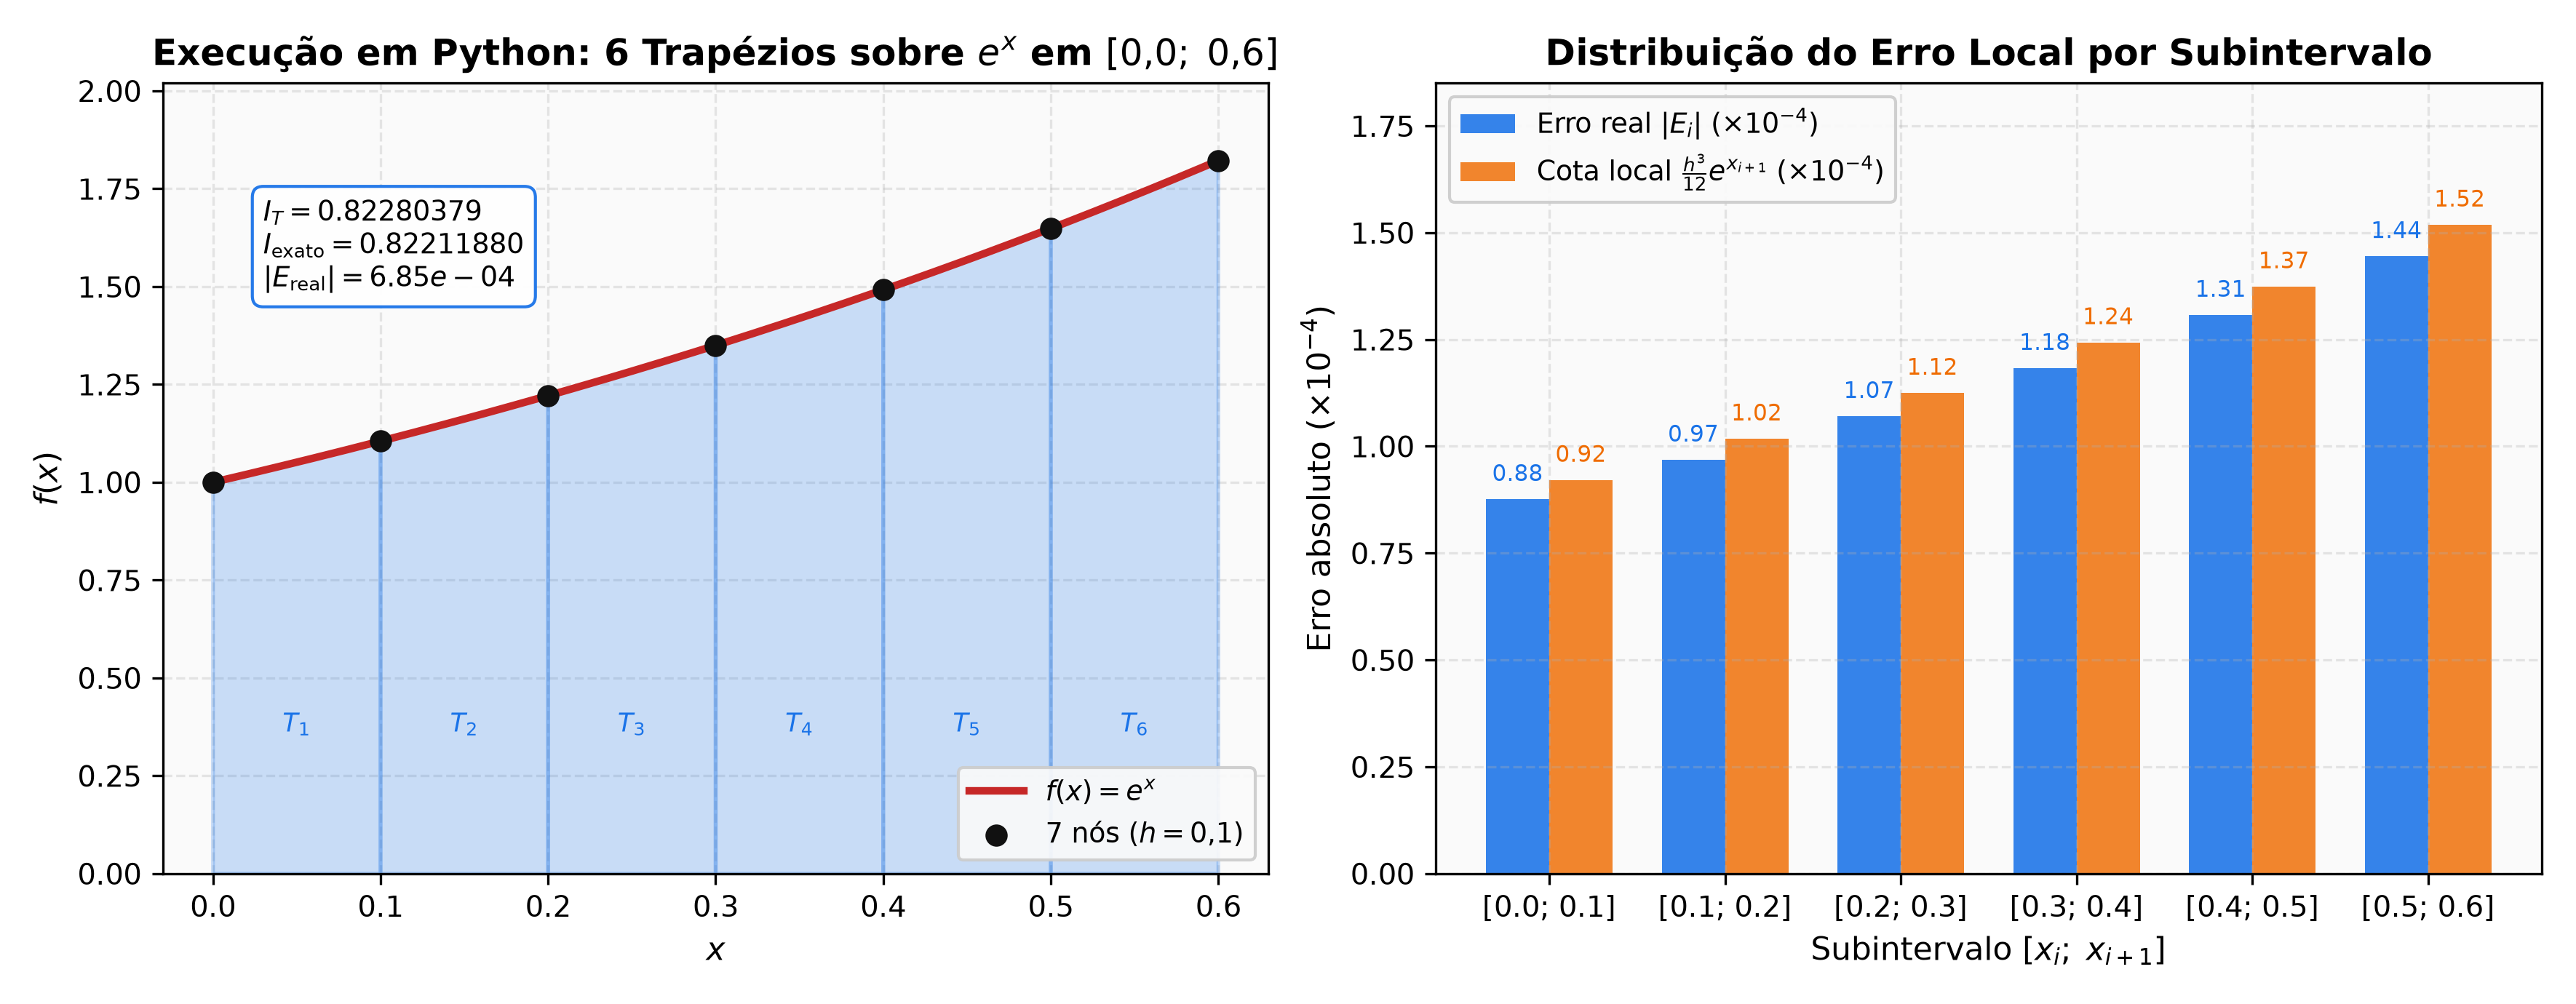
\includegraphics[width=0.93\linewidth]{images/fig_execucao_python_ex.png}
\end{center}
\end{frame}

\begin{frame}{Comportamento do Erro em Python: Convergência Assintótica $O(h^2)$}
\footnotesize
Ao refinar a malha ($n = 1, 2, 3, 6, 12, 24, 48, 96$), a execução em Python comprova empiricamente o decaimento quadrático: cada duplicação de $n$ reduz o erro real por um fator exato de $\approx 4{,}00\times$!

\begin{center}
    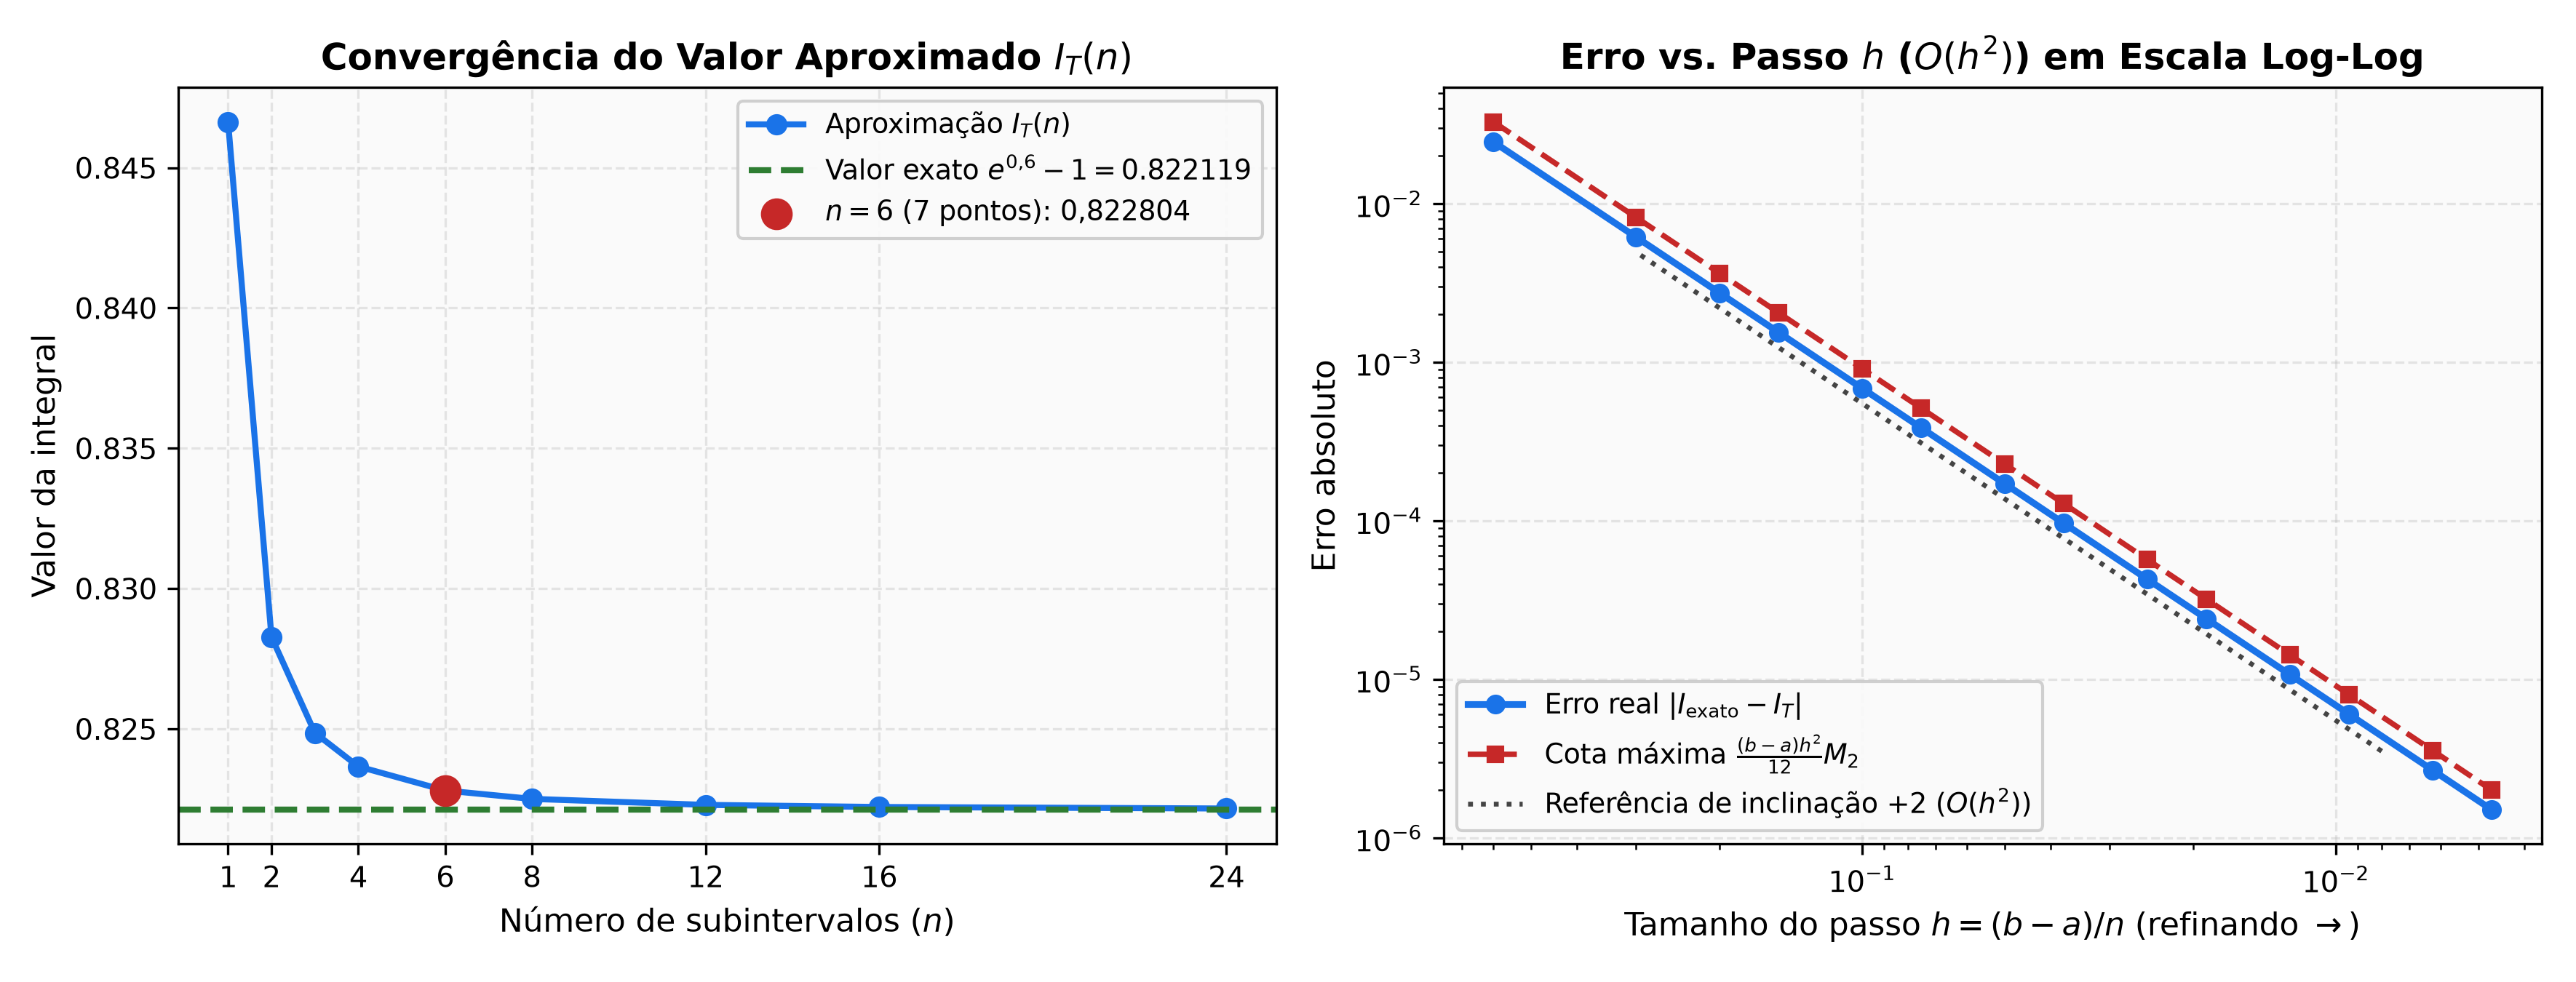
\includegraphics[width=0.93\linewidth]{images/fig_convergencia_erro.png}
\end{center}
\end{frame}

\begin{frame}{Animação em Vídeo: Evolução da Área de Erro com o Refinamento}
\footnotesize
Quadros-chave da animação em vídeo gerada em Python (\code{videos/animacao\_trapezios.mp4} e \code{.gif}), ilustrando visualmente a redução da área residual hachurada conforme $n$ cresce de $1$ até $24$:

\begin{center}
    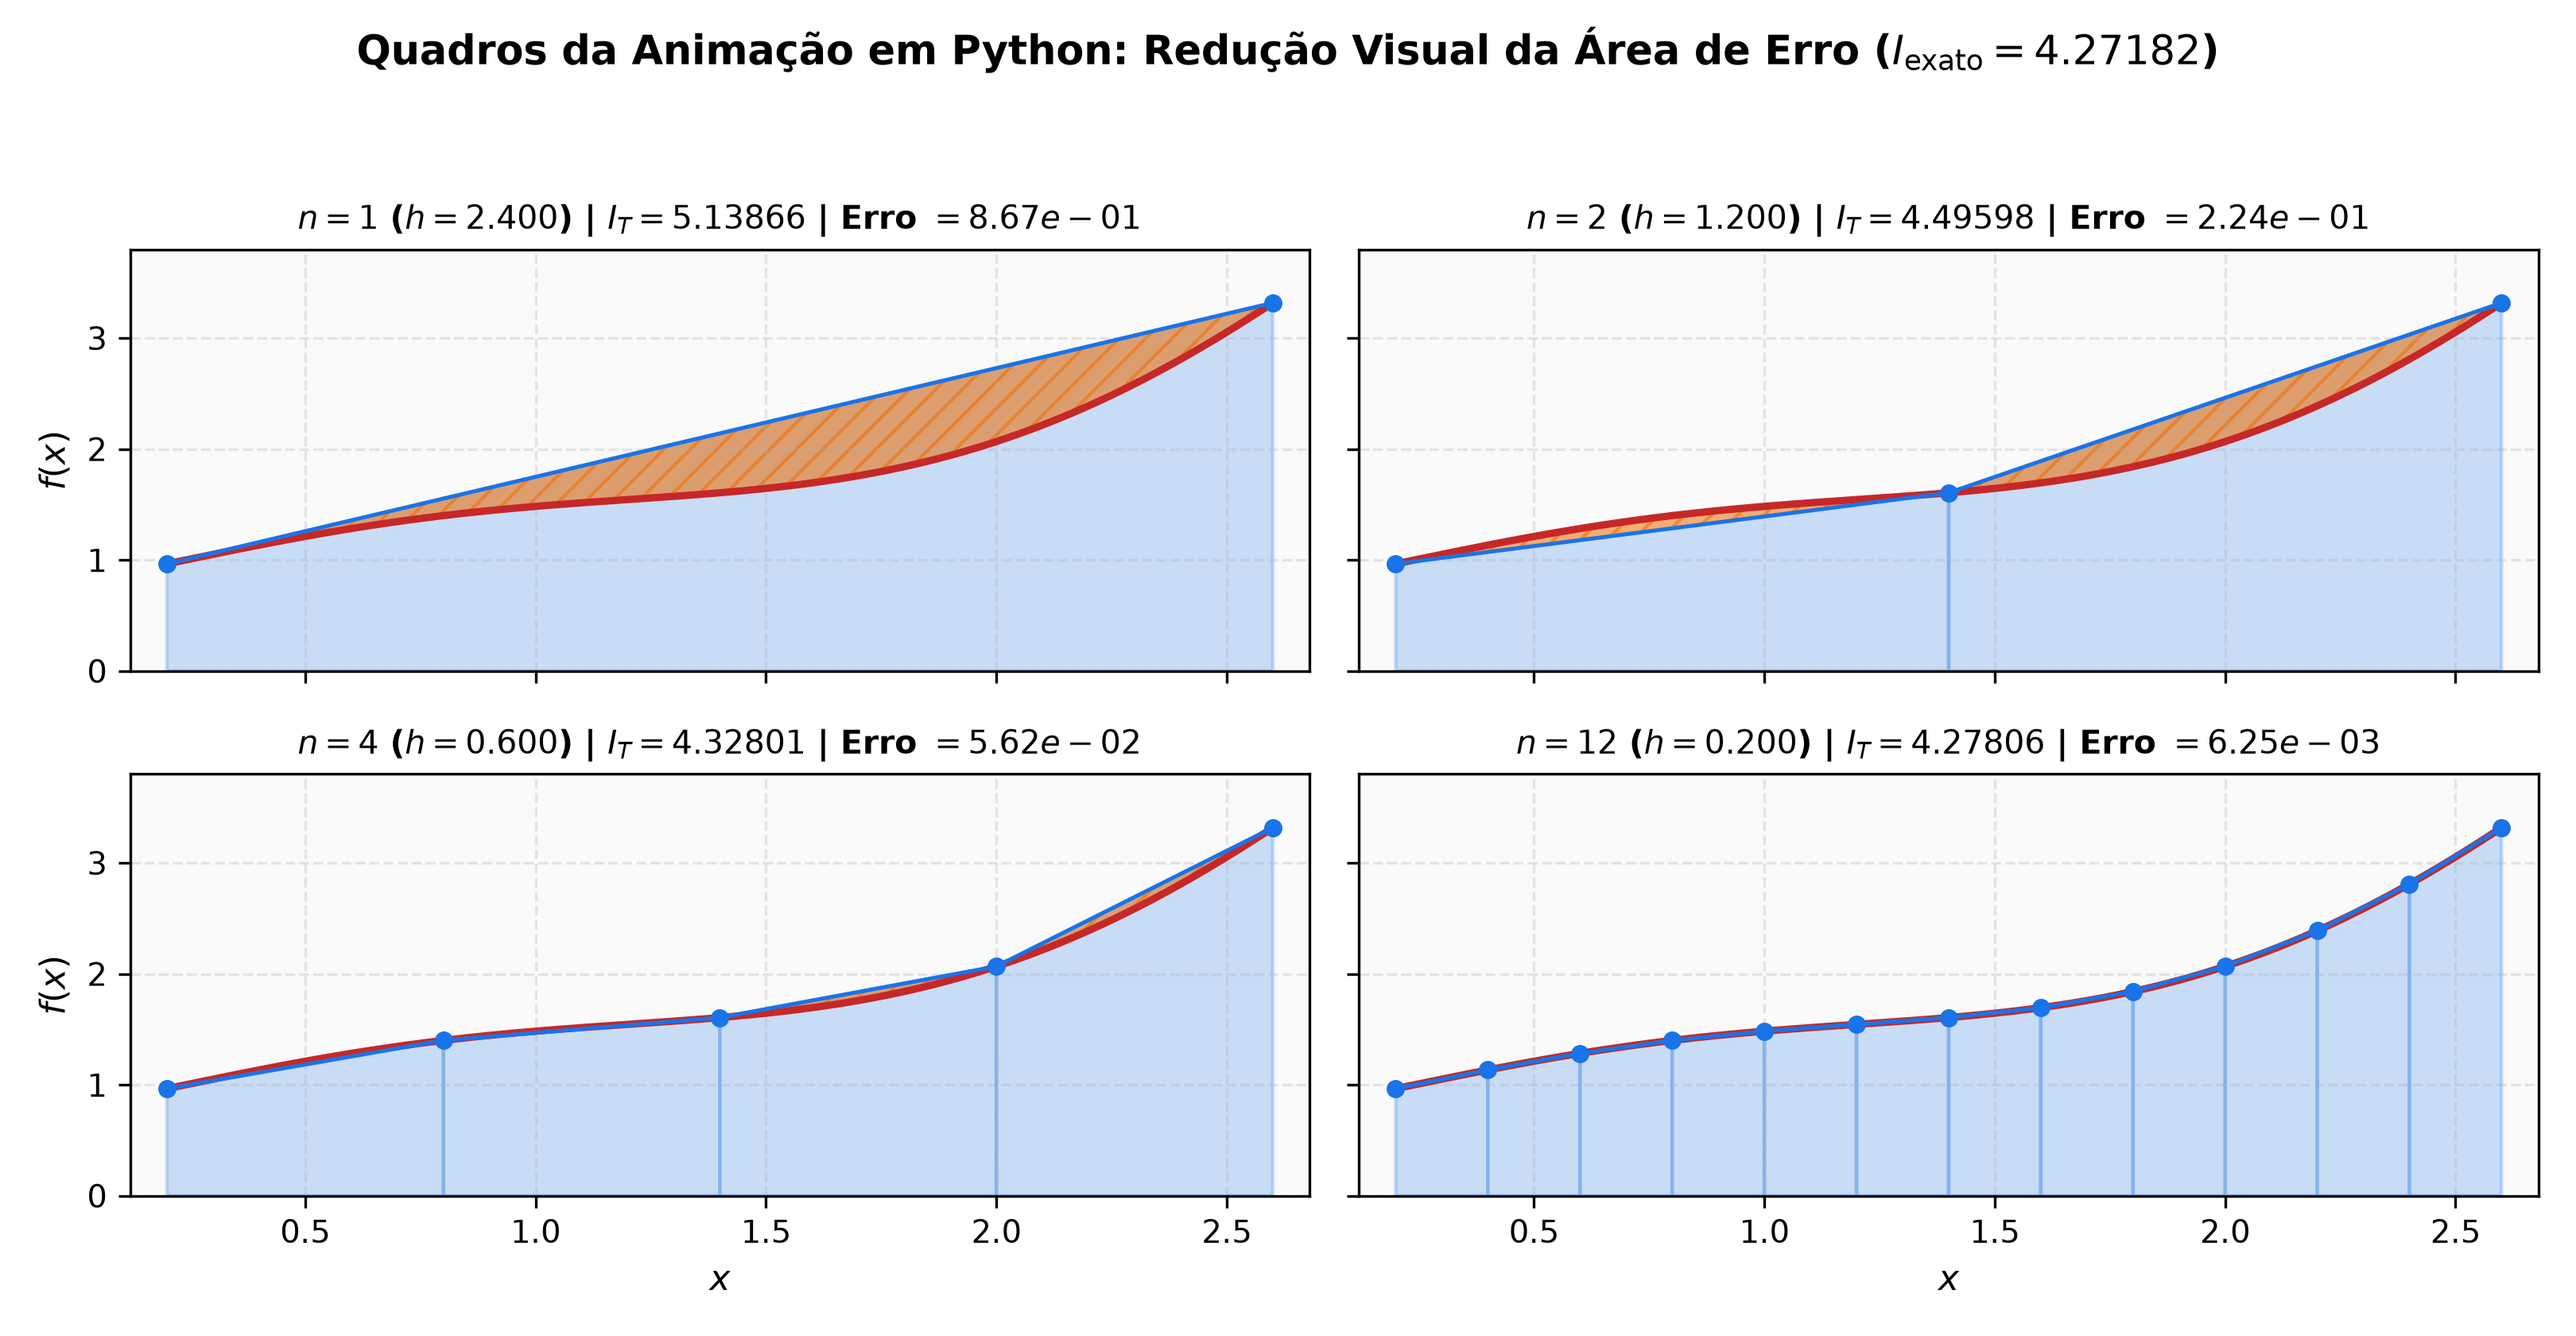
\includegraphics[width=0.80\linewidth]{images/fig_animacao_frames.png}
\end{center}
\vspace{-0.2cm}
\begin{center}
\tiny
\textbf{Acesso ao Vídeo}: \href{run:videos/animacao_trapezios.mp4}{\highlight{Reproduzir vídeo local (\nolinkurl{videos/animacao_trapezios.mp4})}} $\;\bullet\;$
\href{https://github.com/Zuluke/numerical-calculus.git}{\highlight{GitHub (Vídeos e Scripts): \nolinkurl{https://github.com/Zuluke/numerical-calculus.git}}}
\end{center}
\end{frame}

% ============================================================
% SEÇÃO 5: DESAFIO PRÁTICO, MATERIAIS EXTRAS E PRÓXIMA AULA
% ============================================================
\section{Desafio Prático, Materiais Extras e Próxima Aula}

\begin{frame}{Desafio Extra para Prática em Casa: Integral Gaussiana sem Primitiva}
\footnotesize
\begin{bee}[\small Enunciado do Desafio Individual]
A integral $\int_0^1 e^{-x^2}\,dx$ não possui primitiva elementar em funções usuais (define a função erro $\frac{\sqrt{\pi}}{2}\operatorname{erf}(1) \approx 0{,}74682413$). Sabendo que $|f''(x)| = |(4x^2 - 2)e^{-x^2}| \le M_2 = 2$ em $[0, 1]$, determine o menor $n$ que garante $|T_t| \le \varepsilon = 10^{-5}$ e implemente em Python \cite{chapra2016, cardoso2026_github}.
\end{bee}

\begin{bee}[\small Pseudocódigo Estruturado: Dimensionamento Automático e Quadratura]
\begin{algorithmic}[1]\scriptsize
\State \textbf{Entrada:} função $f$, limites $a, b$, limitante $M_2 = \max_{[a,b]} |f''(x)|$, tolerância $\varepsilon > 0$
\State $n \gets \lceil \sqrt{(b - a)^3 \cdot M_2 / (12 \cdot \varepsilon)} \rceil$ \Comment{Cota teórica $a\;priori$}
\State $h \gets (b - a) / n$
\State $S \gets \frac{1}{2}\big(f(a) + f(b)\big)$ \Comment{Contribuição dos nós extremos}
\For{$i \gets 1$ \textbf{até} $n - 1$}
    \State $S \gets S + f(a + i \cdot h)$ \Comment{Acumula nós internos com peso $1$}
\EndFor
\State \textbf{Retornar} $n$, $I_T \gets h \cdot S$
\end{algorithmic}
\end{bee}
\end{frame}

\begin{frame}[fragile]{Solução Comentada do Desafio e Quiz Interativo (15 Questões)}
\scriptsize
\begin{columns}[T]
\begin{column}{0.56\textwidth}
\begin{lstlisting}[language=Python]
import math, numpy as np

a, b, M2, tol = 0.0, 1.0, 2.0, 1e-5
n_min = math.ceil(math.sqrt(((b - a)**3 * M2) / (12 * tol)))

h = (b - a) / n_min
x = np.linspace(a, b, n_min + 1)
y = np.exp(-x**2)
I_T = h * (0.5 * (y[0] + y[-1]) + np.sum(y[1:-1]))
I_ref = 0.5 * math.sqrt(math.pi) * math.erf(1.0)

print(f"n_min = {n_min}, h = {h:.6f}")
print(f"I_T = {I_T:.8f} | Erro = {abs(I_ref - I_T):.2e}")
\end{lstlisting}
\begin{bee}[\small Saída Esperada (Validada em Python)]
\code{n\_min = 130, h = 0.007692 | I\_T = 0.74682050 | Erro = 3.63e-06 <= 1e-05}
\\{\tiny (Obs.: para $\varepsilon = 10^{-4}$, o menor número de subintervalos seria $n_{\min} = 41$, com $I_T = 0{,}74678766$.)}
\end{bee}
\end{column}

\begin{column}{0.44\textwidth}
\begin{bee}[\small Lista de Exercícios em Quiz Interativo]
\begin{itemize}\scriptsize
    \item Acesse o arquivo \highlight{\code{quiz\_aula\_MT.html}} em seu navegador!
    \item Contém \textbf{15 questões objetivas} (conceituais e de cálculo numérico passo a passo) com:
    \begin{itemize}\tiny
        \item Dicas pedagógicas orientadas;
        \item Feedback imediato ao confirmar;
        \item Gabarito completo detalhado justificando todas as alternativas.
    \end{itemize}
\end{itemize}
\end{bee}
\end{column}
\end{columns}
\end{frame}

\begin{frame}{Materiais Extras, Vídeoaulas e Hyperlinks Explícitos}
\footnotesize
\begin{bee}[\small Repositórios, Notas de Aula e Vídeoaulas Recomendadas]
\begin{itemize}\scriptsize
    \item \textbf{Repositório GitHub do Curso (Scripts Python, Figuras e Vídeos)}: \\
    \href{https://github.com/Zuluke/numerical-calculus.git}{\nolinkurl{https://github.com/Zuluke/numerical-calculus.git}} \cite{cardoso2026_github}
    \item \textbf{Portal de Métodos Numéricos --- CIn/UFPE (Prof. Rafael Mesquita)}: \\
    \href{https://cin.ufpe.br/~rgm/metodosnumericos/}{\nolinkurl{https://cin.ufpe.br/~rgm/metodosnumericos/}} \cite{mesquita2026}
    \item \textbf{Disciplina MS211 --- Cálculo Numérico (IMECC/UNICAMP)}: \\
    \href{https://disciplinas.ime.unicamp.br/ms211/ementa/}{\nolinkurl{https://disciplinas.ime.unicamp.br/ms211/ementa/}} \cite{unicamp_ms211}
    \item \textbf{Vídeoaula 1 [PT-BR] --- UNIVESP (Integração Numérica e Regra dos Trapézios)}: \\
    \href{https://www.youtube.com/playlist?list=PLxI8Can9yAHdCutIICyWcGI0s-fbpw3fc}{\nolinkurl{https://www.youtube.com/playlist?list=PLxI8Can9yAHdCutIICyWcGI0s-fbpw3fc}} \cite{univesp_video}
    \item \textbf{Vídeoaula 2 [EN] --- Khan Academy (Trapezoidal Approximation \& Error)}: \\
    \href{https://www.youtube.com/watch?v=1p0NHR5w0Lc}{\nolinkurl{https://www.youtube.com/watch?v=1p0NHR5w0Lc}} \cite{khan_trapezoid_video}
    \item \textbf{Documentação SciPy (\code{scipy.integrate.trapezoid})}: \\
    \href{https://docs.scipy.org/doc/scipy/reference/generated/scipy.integrate.trapezoid.html}{\nolinkurl{https://docs.scipy.org/doc/scipy/reference/generated/scipy.integrate.trapezoid.html}} \cite{scipy_trapezoid}
\end{itemize}
\end{bee}
\end{frame}

\begin{frame}{Próxima Aula: Método de Simpson ($1/3$ e $3/8$) e Comparação de Erros}
\footnotesize
Como vimos, o Método dos Trapézios aproxima $f(x)$ por \textbf{retas} ($n=1$ em Newton-Cotes), resultando em erro de ordem $O(h^2)$. Na próxima aula, daremos um salto de precisão substituindo retas por \highlight{parábolas} e \highlight{cúbicas} \cite{santos2010, mesquita2026, burden2016}:

\begin{center}
\begin{tabular}{lcccc}
\toprule
\textbf{Método (Newton-Cotes)} & \textbf{Grau Local} & \textbf{Restrição de $n$} & \textbf{Cota do Erro Global} & \textbf{Erro em $\int_{0{,}0}^{0{,}6} e^x\,dx$ ($n=6$)} \\
\midrule
Trapézios (Hoje) & $1$ (Retas) & Qualquer $n \ge 1$ & $\frac{n h^3}{12} M_2 = O(h^2)$ & $\le 9{,}1106 \times 10^{-4}$ \\
\rowcolor{primary!10}
\textbf{$1/3$ de Simpson (Próxima)} & $2$ (Parábolas) & \textbf{$n$ deve ser par} & $\frac{n h^5}{180} M_4 = O(h^4)$ & $\le 6{,}0737 \times 10^{-7}$ \\
$3/8$ de Simpson (Próxima) & $3$ (Cúbicas) & $n$ múltiplo de $3$ & $\frac{n h^5}{80} M_4 = O(h^4)$ & $\le 1{,}3666 \times 10^{-6}$ \\
\bottomrule
\end{tabular}
\end{center}
\vspace{0.15cm}
\begin{bee}[\small Ganho de Precisão com os Mesmos 7 Pontos]
A simples troca de segmentos de reta por arcos parabólicos reduz a cota máxima do erro em \highlight{1.500 vezes} ($9{,}11\times 10^{-4} \rightarrow 6{,}07\times 10^{-7}$) sem aumentar o custo de avaliação da função!
\end{bee}
\end{frame}

% ============================================================
% REFERÊNCIAS BIBLIOGRÁFICAS (SEM \section{} ANTES)
% ============================================================
\begin{frame}[allowframebreaks]{Referências Bibliográficas}
\nocite{*}
\printbibliography
\end{frame}

\begin{frame}
    \centerline{\Huge OBRIGADO!}
    \vspace{0.5cm}
    \centerline{\Large Perguntas e Discussões}
    \vspace{0.3cm}
    \centerline{\small Prof. João Cardoso $\;\bullet\;$ Cálculo Numérico}
    \vspace{0.2cm}
    \centerline{\footnotesize Próxima Aula: Método de Simpson ($1/3$ e $3/8$) e Análise Comparativa de Erros.}
    \vspace{0.25cm}
    \centerline{\tiny \href{https://github.com/Zuluke/numerical-calculus.git}{\nolinkurl{https://github.com/Zuluke/numerical-calculus.git}}}
\end{frame}

\end{document}
